%!TEX root = ../master.tex
\chapter{Evaluation}\label{ch:evaluation}
This chapter will describe the evaluation process of the finished prototype. The chapter is spilt into three subsections: a planning section, actual evaluation description and analysis of evaluation results. 

\section{Further Context}\label{sec:furthercontext}
\todo{additional functionality: draw on image to change the sound} wut?

\section{Planning of evaluation}
This section will describe the thoughts the project group made before the actual evaluation test were made. The section will show a description of the evaluation tasks and question there were planned to be asked during the test. 

"underoverskrift eller noget" 

What do we want out of this test?

\begin{itemize}
\item The user can alter the output by applying filters.
\item The user understands the interface  
\item The prototypes usability is over 80 percent of the users satisfaction.
\end{itemize}

Interview question 
\begin{itemize}
\item What did you experience when manipulating with the sliders?
\item did you 
\item Where you confused about the design?
\item was the “text” helpfull to you?
\item Any other thoughts?
\end{itemize}

Assignments for the user to solve during the test 
\begin{itemize}
\item Turn on echo
\item Turn on echo and comb
\item Turn off comb
\item Turn on bandpass 
\end{itemize}


The test set up was planned to be held in a quiet area with one test participant at the time, located at Rendensburgade (The Create building) it was planned to conduct the test on at least 12 people (2 test people pr. group member) 


Technical evaluation 



\section{Evaluation test}
This section will give a description of the set-up, procedure and results of the actual evaluation test of the final device. 

\begin{figure}[!h] 
\centering
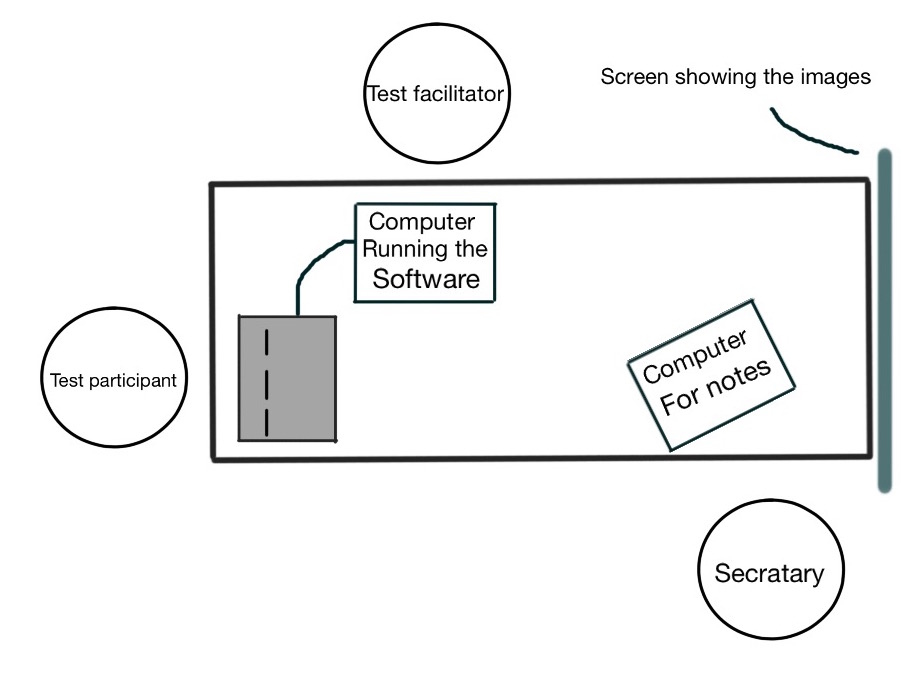
\includegraphics[width=1\textwidth]{testsetup}
\caption{\label{fig:testsetup} Illustration of the test set-up.}
\end{figure}

The final test was conducted on 15 test participants, all students in their 20's.  \todo{dette kan bruges i diskution, da vi ville have fået mere variation i resultaterne hvis vi fx. havde testet på museumsgæster i alle aldre} The test took place in a small closed room located at Rendesburggade (the Create building) A main test facilitator; who interviewed the participants and was in control over the product, and a secretary who took notes of the entire test, was placed in the test location, a screen was also available in the test room, this screen was used to display the two pictures the project group decide to use during the test.

\begin{figure}[!h] 
\centering
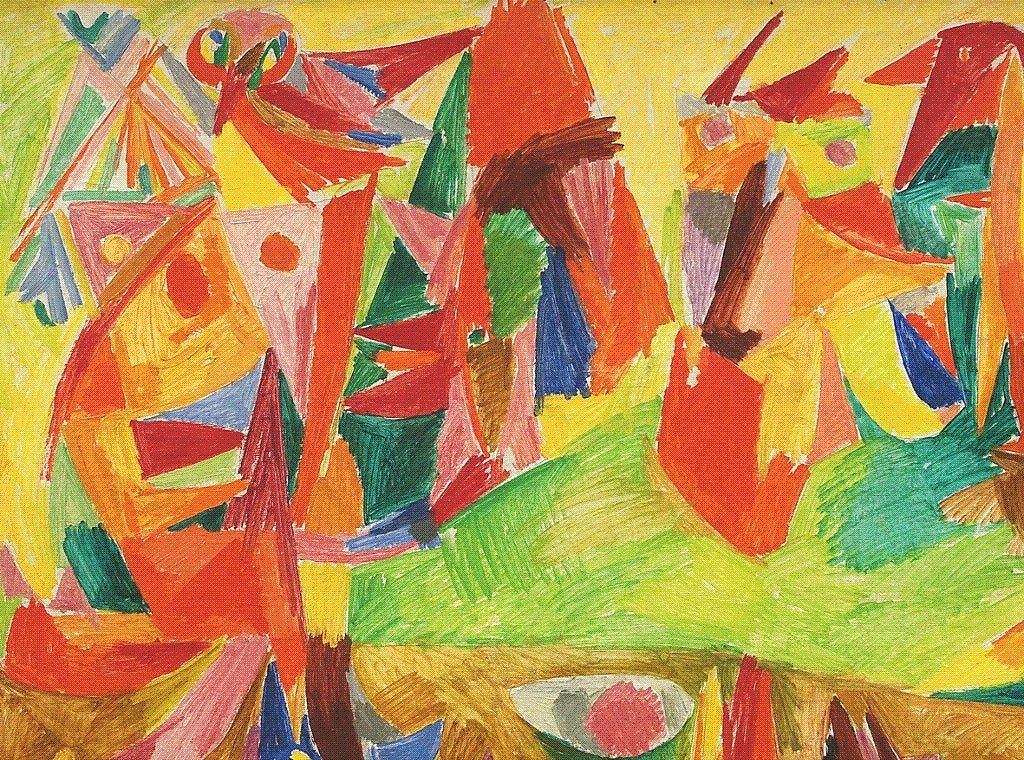
\includegraphics[width=1\textwidth]{asger}
\caption{\label{fig:asger} Asger Jorns "Trolden og Fuglene" 1944.}
\end{figure}

\begin{figure}[!h] 
\centering
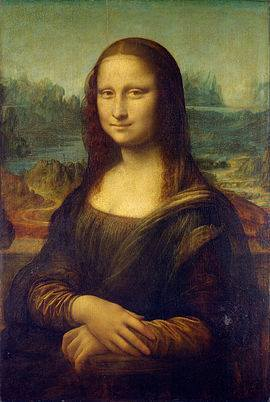
\includegraphics[width=1\textwidth]{monalisa}
\caption{\label{fig:monalisa} Leonardo Da Vinci "Mona Lisa" 1503-1517.}
\end{figure}

The test was carried out by welcoming the test participants in the room, one at the time. The participants were places at the end of the table and was asked to sign a consent form. The facilitator then started the test by introducing the overall project and explaining what the participant is expected to do during the test. The facilitator conducted the test by using the scribt shown below:


\section{Scribt}

Hello and thank you for wanting to participate in this test. We are group 30.

Our prototype takes an image and turns it into a sound. During this test we will give you a few different assignments and ask you questions during the test. This is a test of the product, and we prefer you to think out loud during the test.

//Mona
Questions: 


\begin{itemize}
\item What do you think you have to do with this product?
\item What happens when you manipulated with the sliders?
\item Can you hear a difference between “MIN” and “MAX”?
\item Can you hear a difference between the effects?
\item Is the “help text” helpfull to you?
\item Is the help text clear?
\item Any other thoughts?
\end{itemize}



/* Now we will change the images to Asgar Jorn */
\begin{itemize}
\item Do you hear the difference between the pictures?
\item Why do you think there is a difference between the images?
\item Can you hear a difference between “MIN” and “MAX”?
\item Can you hear a difference between the effects?
\end{itemize}


Any other overall thoughts?


\section{Evaluation results}
\todo{Write the results, describe the general opinion}

From the testing the participants had a general opinion about the interface

\todo{Many of the participants found it difficult to hear the difference when manipulating with the comb filter on both pictures. However when using the Bandpass and High shelf the user could hear a difference in the two when changing the values using the sliders. The participants were not certain what the filters did since they had never seen them before, but they could distinguish a change in the volume when manipulating with the sliders. Moreover the interface was clear for the participants and how to use it. 

One particpant was asking if the later iteration would show the context between the picture and sound to find a balanced and satisfying output. }